\documentclass[11pt]{article}

\setlength{\oddsidemargin}{-0.25 in}
\setlength{\evensidemargin}{-0.25 in}
\setlength{\topmargin}{-0.9 in}
\setlength{\textwidth}{7.0 in}
\setlength{\textheight}{9.0 in}
\setlength{\headsep}{0.75 in}
\setlength{\parindent}{0.3 in}
\setlength{\parskip}{0.1 in}
\usepackage{epsf}
\usepackage{pseudocode}
\usepackage{amsmath}
\usepackage{amssymb}
\usepackage[normalem]{ulem}
\usepackage{graphicx}
\usepackage[export]{adjustbox}
\pagenumbering{gobble}
\def\O{\mathop{\smash{O}}\nolimits}
\def\o{\mathop{\smash{o}}\nolimits}
\newcommand{\e}{{\rm e}}
\newcommand{\R}{{\bf R}}
\newcommand{\Z}{{\bf Z}}

\title{Section 2: Search}
\author{CS 182 - Artificial Intelligence}
\date{}
\begin{document}
\maketitle


\renewcommand{\labelenumii}{\arabic{enumii}.}
\setlength{\parindent}{0pt}

A \textbf{search problem} can be defined by the tuple
$(S, A, R, C, S_0, G)$, where
\begin{itemize}
\item $S$ represents the set of possible \underline{states}

\item $A$ represents the set of possible \underline{actions}, which may vary
from state to state

\item $R : S \times A \rightarrow S$ is the \underline{transition model},
which represents the result of actions from a state

\item $C : S \times A \rightarrow \mathbb{R}$ represents the \underline{cost}
of taking an action

\item $S_0$ represents the \underline{starting state}

\item $G$ represents the \underline{goal test}, the set of {goal states}
\end{itemize}

Together, these parameters implicitly form a \underline{state space graph},
where nodes are possible states and edges are actions connecting states.

\underline{Tree search} is a method of exploring a state space graph by expanding out potential plans. Tree search builds a tree of searched states and maintains a \underline{fringe} of partial plans under consideration. The objective is to find a plan that reaches the goal state, and it is ideal to try to expand as few nodes as possible on the state space graph.

\underline{Graph search} extends tree search to account for state space graphs with cycles by keeping a set of visited nodes. These visited nodes are not explored again, avoiding repeated work.

\textbf{Uninformed Search:}
\vspace{-10pt}
\begin{itemize}
\item \underline{Depth-First Search ({DFS})} maintains the fringe as a stack and expands the ``deepest'' nodes first.

\item \underline{Breadth-First Search ({BFS})} maintains the fringe as a queue and expands the ``shallowest'' nodes first.

\item \underline{Uniform Cost Search ({UCS})} maintains the fringe as a priority queue ordered by the cumulative cost of a path. UCS is optimal for all edge costs $>0$.

\end{itemize}

\textbf{Informed Search:}
\vspace{-10pt}
\begin{itemize}
\item \underline{Greedy Search }maintains the fringe as a priority queue ordered by a heuristic function $h(x)$ that maps states to estimated distance to goal.

\item \underline{A* Search extends} greedy search and maintains the fringe as a priority queue ordered by summing the cumulative cost of a path to state $x$, $g(x)$, and the heuristic at $x$, $h(x)$ aka
$f(x) = g(x) + h(x)$.

\newpage
Psuedocode for both Tree and Graph search are shown below. Note: the frontier referenced below is the fringe. Think about how using a different data structure for the fringe would allow each of the algorithms to execute the above search algorithms.

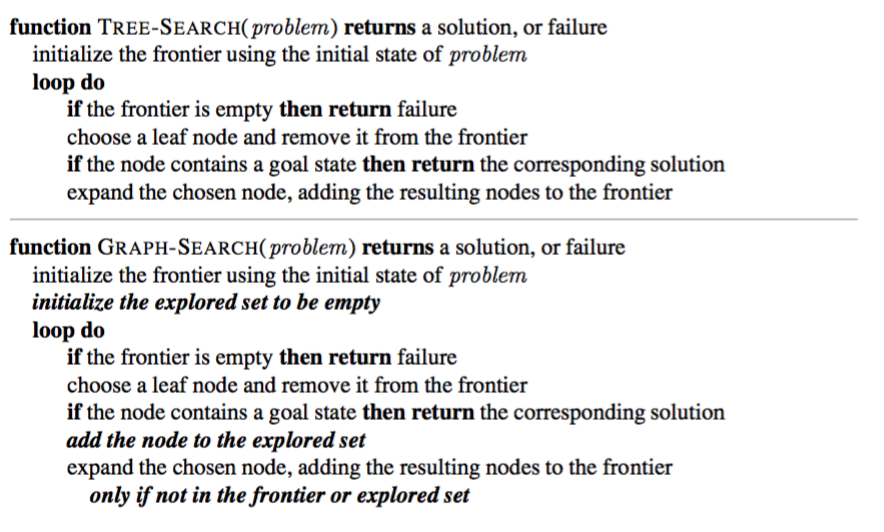
\includegraphics{img/search}

\textbf{Heuristics:}

A heuristic function is used to estimate the cost of reaching a goal
from a state in the state space.

A heuristic $h$ is \underline{admissible} if it never overestimates the cost
of reaching the goal, i.e. $\forall x, h(x) \le h^*(x)$ where
$h^*$ is the optimal cost to reach the goal.

A heuristic $h$ is \underline{consistent} if it never overestimates
the estimated distance to the goal of a neighbor plus
the cost of reaching the neighbor, i.e.
$\forall x, h(x) \le c(x, x') + h(x')$

\end{itemize}

\newpage

\begin{enumerate}

\item
% \emph{Review.} Consider the 8-puzzle, where tiles adjacent to blank spaces
% can slide into the blank spaces, until the puzzle is rearranged to fit the
% goal state. Describe each element of a search problem for solving this puzzle. (AIMA)
Consider the Tower of Hanoi puzzle, where a stack of disks
must be moved from the leftmost peg to the rightmost peg, while maintaining
the invariant that no disk may be placed on top of a smaller disk.
Describe each element of a
search problem for solving this puzzle. How many possible states are in
this representation? (Image: Popular Science Monthly Vol. 26)

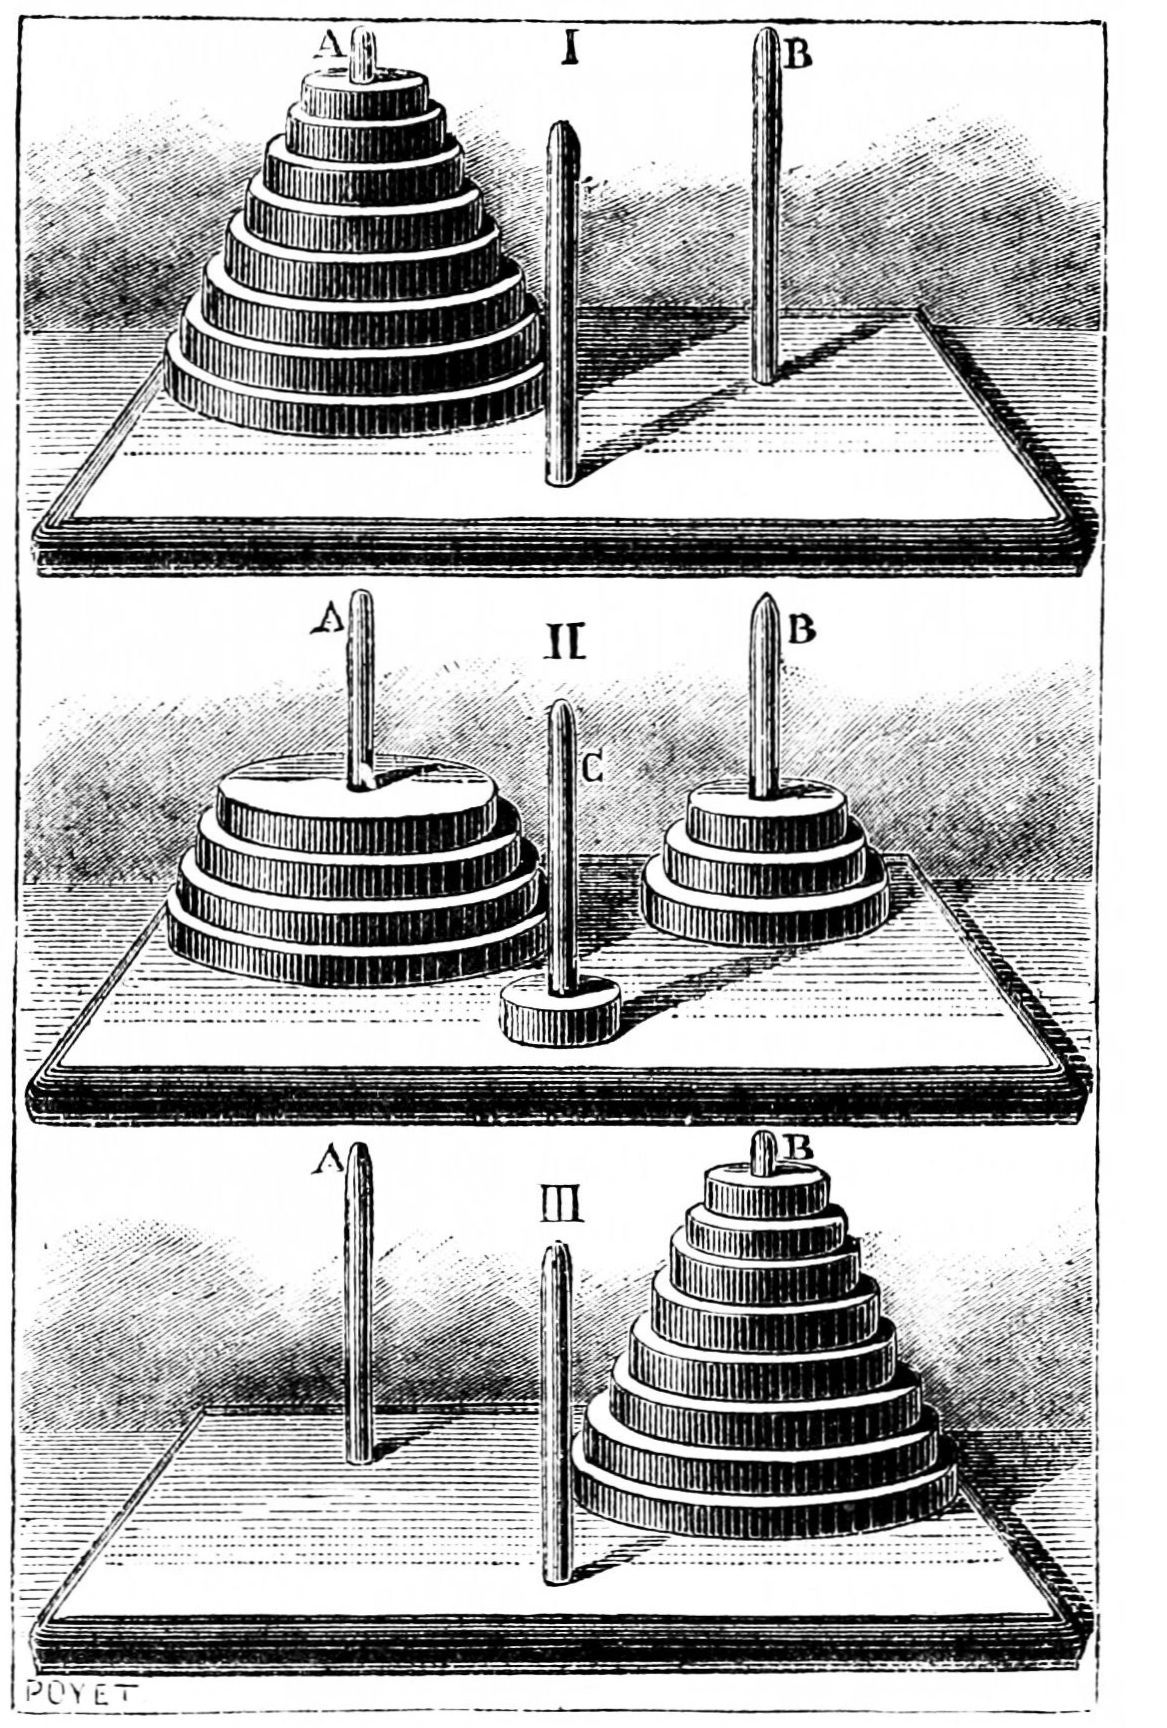
\includegraphics[scale=0.15, right]{img/hanoi}

\item
Consider the 8 queens puzzle, where queens must be placed on a
chessboard so they do not attack each other. Describe each element of a
search problem for solving this puzzle. How many possible states are in
this representation? (AIMA)

\begin{figure}[h!t]
  \centering
  \caption{A nearly-complete 8-queens puzzle solution}
  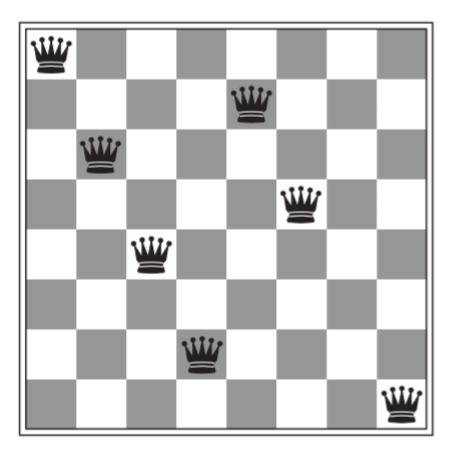
\includegraphics{img/8queens}
\end{figure}

\item Can you think of another, more compact representation of the state space? (AIMA)
% How many possible states are in this representation?

\newpage
\item
You are programming a holiday shopping robot that will drive from store to
store in order to buy all the gifts on your shopping list.  You have a set
of $N$ gifts $G = \{ g_1 ,g_2 ,...g_N \}$ that must be purchased.  There are
$M$ stores, $S = \{ s_1 ,s_2 ,...s_M \}$ each of which stocks a known inventory
of items:  we write $g_k \in s_i$ if store $s_i$ stocks gift $g_k$. Shops may
cover more than one gift on your list and will never be out of the items they
stock.  Your home is the store $s_1$, which stocks no items.

The actions you will consider are travel-and-buy actions
in which the robot travels from its current location $s_i$ to another
store $s_j$ in the fastest possible way and buys whatever items remaining on
the shopping list that are sold at $s_j$.  The time to travel-and-buy from
$s_i$ to $s_j$ is $t(s_i,s_j)$.  You may assume all travel-and-buy actions
represent shortest paths, so there is no faster way to get between
$s_i$ and $s_j$ via some other store.  The robot begins at your home with no
gifts purchased.  You want it to buy all the items in as short a time as
possible and return home.

For this planning problem, you use a state space where each state is a pair
$(s,u)$ where $s$ is the current location and $u$ is the set of unpurchased
gifts on your list (so $g \in u$ indicates that gift $g$ has not yet been purchased).
(Berkeley CS 188, Fall 2011)

How large is the state space in terms of the quantities defined above?

\bigskip \bigskip \bigskip \bigskip
\bigskip \bigskip \bigskip \bigskip
\bigskip \bigskip \bigskip \bigskip

\item You have waited until very late to do your shopping, so you decide to send an swarm of
$R$ robot minions to
shop in parallel.  Each robot moves at the same speed, so the same
store-to-store times apply.  The problem
is now to have all robots start at home, end at home, and for each item
to have been bought by at least one
robot (you don’t have to worry about whether duplicates get bought).
Hint:  consider that robots may not all
arrive at stores in sync. (Berkeley CS 188, Fall 2011)

Give a minimal state space for this search problem:

\newpage

\item Consider the search graph shown below.
$S$ is the start state and $G$ is the goal state. All edges are bidirectional. For each of the following \underline{graph} search strategies, give the path that would be returned, or write none if no path will be returned. If there are any ties, assume alphabetical tiebreaking (i.e., nodes for states earlier in the alphabet are expanded first in the case of ties). \\(Berkeley CS 188, Fall 2011)

{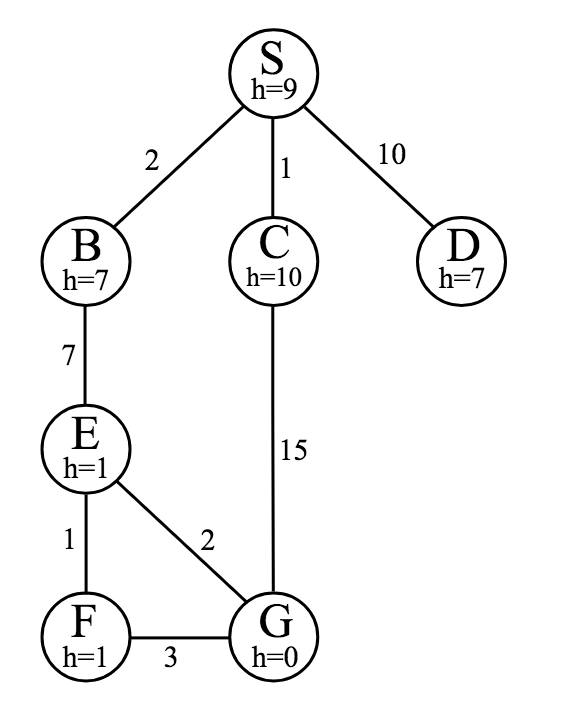
\includegraphics[scale=0.7, center]{img/tree2}}

\begin{itemize}
\item DFS

\bigskip
\bigskip
\item BFS

\bigskip
\bigskip
\item UCS

\bigskip
\bigskip
\item Greedy Search

\bigskip
\bigskip
\item A* Search
\end{itemize}

\newpage

\item
Consider the state space graph shown below in which some of the states are missing a heuristic value. \\ (Berkeley CS 188, Spring 2015)

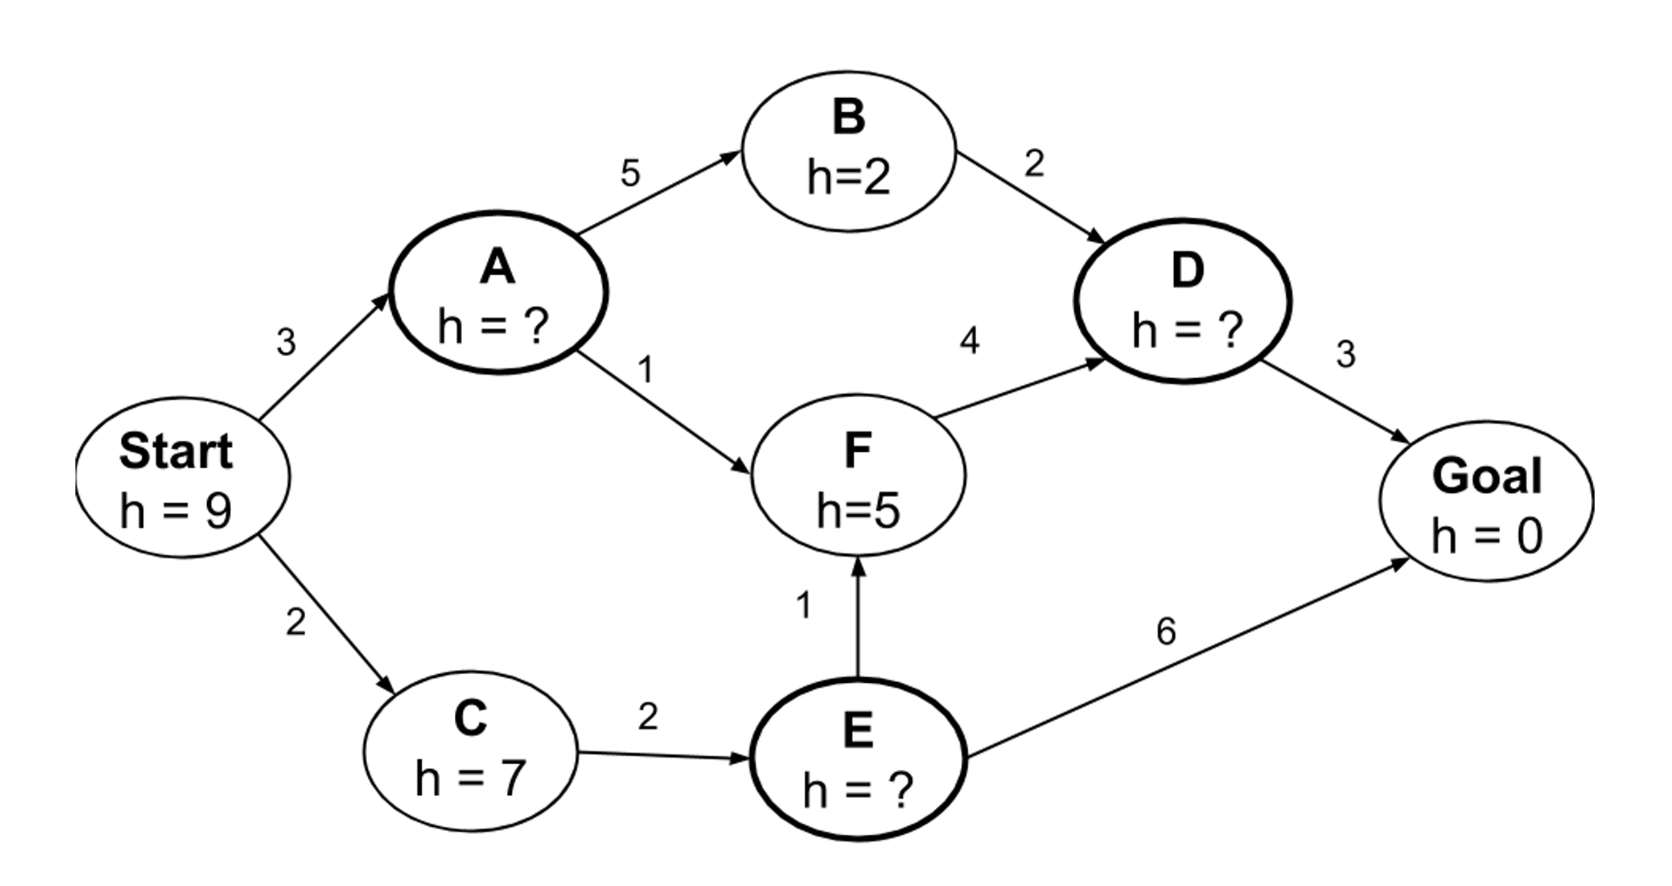
\includegraphics[width=\textwidth]{img/Heuristics}

Determine the possible range for each missing heuristic value so that the heuristic is admissible. 
\\ \\ \\ \\ \\ \\ \\ \\ \\

Additionally, for what range of each heuristic value is the heuristic consistent?
\\ \\ \\ \\ \\ \\ \\ \\ \\

\newpage
\item
The heuristic path algorithm (Pohl, 1977) is a best-first search in which the evaluation function is $f(n) = (2 ~ -w)g(n) + wh(n)$. (AIMA)
\\ \\
For what values of $w$ is this optimal, assuming that $h$ is admissible?
\\ \\ \\ \\ \\ \\ \\ \\ \\
What kind of search does this perform for $w = 0$, $w = 1$, and $w = 2$?
\\ \\ \\ \\ \\ \\ \\ \\ \\ \\ \\ \\

\item
For the Tower of Hanoi puzzle from before, come up with an admissible
heuristic function.
\end{enumerate}

\newpage


\clearpage
\clearpage
\end{document}
